%%%%%%%%%%%%%%%%%%%%%%%%%%%%%%%%%%%%%%%%%%%%%%%%%%%%%%%%%%%%%%%%%%%%%%%%%%%

\documentclass{standalone}

\usepackage{mathptmx}
\usepackage{tikz}
\usetikzlibrary{angles}
\usetikzlibrary{external}
\tikzexternalize{pendulum}

%% We default to Times.
\renewcommand{\rmdefault}{ptm}
\renewcommand{\ttdefault}{pcr}
%% Enable Times/Palatino main text font.
\normalfont\selectfont

%% The pendulum.
\newcommand{\genericPoint}{%%
  %% Highlight the trajectory of the pendulum.
  \draw[red,thick,<->,dashed] (origin) ++ (A) arc[radius=\radius,start angle=240,end angle=300];
  %% Vertical line perpendicular to horizontal axis.
  \draw[dashStyle] (origin) -- (0,-\radius);
  %% The cord of the pendulum.
  \radiusLine
  %% The bob of the pendulum.
  \shade[ball color=gray] (\xa,\yb) circle (5pt);
  %% The horizontal platform.
  \draw[fill=gray!50] (-0.5,0) rectangle (0.5,0.2);
}

%% The radius.
\newcommand{\radiusLine}{%%
  %% A line as the radius
  \draw[lineStyle] (origin) -- (point);
  %% Label the angle.
  \path pic[draw,->,thick,angle radius=1cm] {angle=xyRadius--origin--point};
  \node at (0.2,-1.25) {$\varphi$};
}


%%%%%%%%%%%%%%%%%%%%%%%%%%%%%%%%%%%%%%%%%%%%%%%%%%%%%%%%%%%%%%%%%%%%%%%%%%%
%% A disc of radius 6 cm.
%%%%%%%%%%%%%%%%%%%%%%%%%%%%%%%%%%%%%%%%%%%%%%%%%%%%%%%%%%%%%%%%%%%%%%%%%%%

\begin{document}

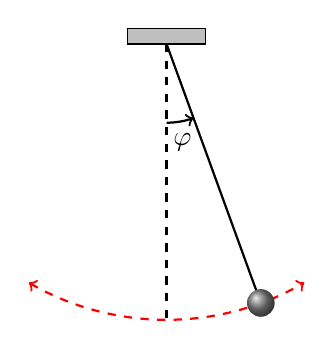
\begin{tikzpicture}[%%
  dashStyle/.style={-,thick,dashed},%%
  lineStyle/.style={-,thick},%%
]
%%
%%
\pgfmathsetmacro{\radius}{3.5}
\pgfmathsetmacro{\xa}{1.19707050163984}
\pgfmathsetmacro{\yb}{-3.28892417275068}
%% The Cartesian coordinate system.
\coordinate (A) at (-1.75,-3.03108891324554);
\coordinate (origin) at (0,0);
%% The generic angle.
\coordinate (point) at (\xa,\yb);
\coordinate (xyRadius) at (0,-\radius);
%%
%%
%% Illustrate a circle.
\genericPoint
\end{tikzpicture}

\end{document}
